\begin{figure}[H]
\begin{subfigure}[c]{0.46\textwidth}
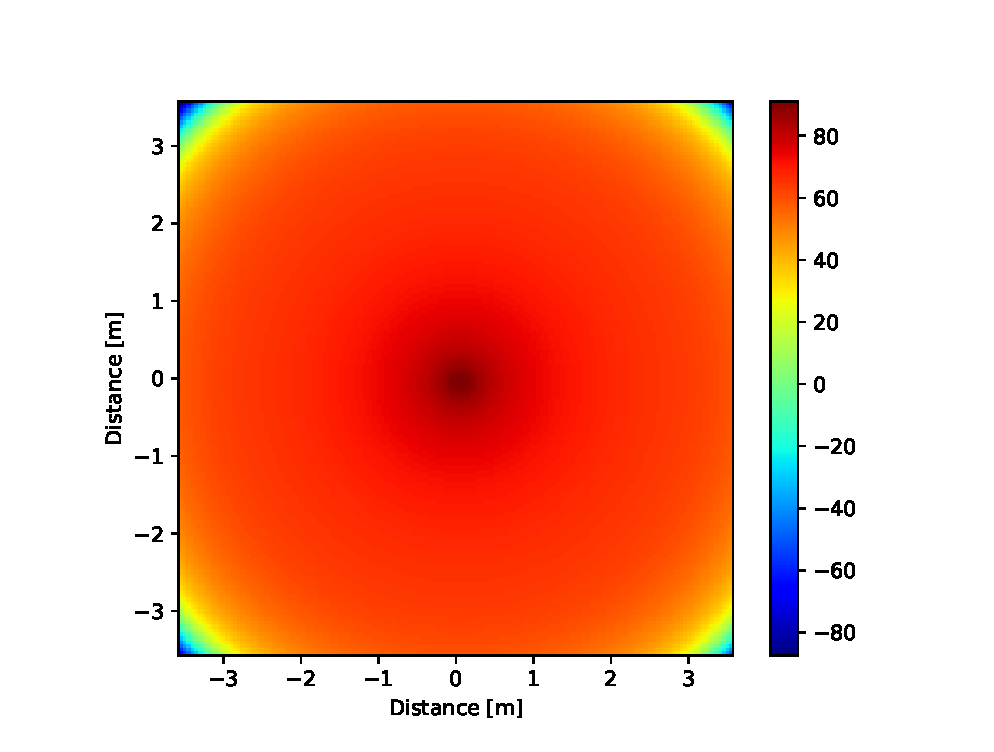
\includegraphics[width=1\textwidth]{p_rms_10m_32.eps}
\subcaption{$D=\SI{10}{\meter}$, single precision}
\label{fig:p_rms_10m_32}
\vspace{5mm}
\end{subfigure}
\hfill
\begin{subfigure}[c]{0.46\textwidth}
\includegraphics[width=1\textwidth]{p_rms_10m_64.eps}
\subcaption{$D=\SI{10}{\meter}$, double precision}
\label{fig:p_rms_10m_64}
\vspace{5mm}
\end{subfigure}
\begin{subfigure}[c]{0.46\textwidth}
\includegraphics[width=1\textwidth]{p_rms_20m_32.eps}
\subcaption{$D=\SI{20}{\meter}$, single precision}
\label{fig:p_rms_20m_32}
\vspace{5mm}
\end{subfigure}
\hfill
\begin{subfigure}[c]{0.46\textwidth}
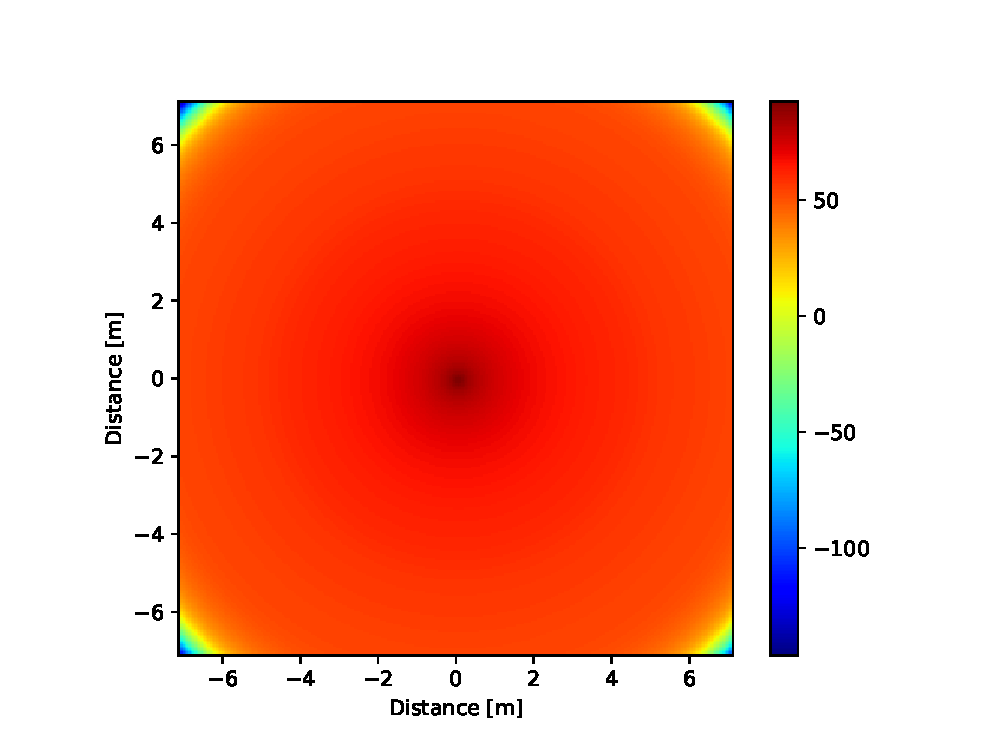
\includegraphics[width=1\textwidth]{p_rms_20m_64.eps}
\subcaption{$D=\SI{20}{\meter}$, double precision}
\label{fig:p_rms_20m_64}
\vspace{5mm}
\end{subfigure}
\begin{subfigure}[c]{0.46\textwidth}
\includegraphics[width=1\textwidth]{p_rms_30m_32.eps}
\subcaption{$D=\SI{30}{\meter}$, single precision}
\label{fig:p_rms_30m_32}
\vspace{5mm}
\end{subfigure}
\hfill
\begin{subfigure}[c]{0.46\textwidth}
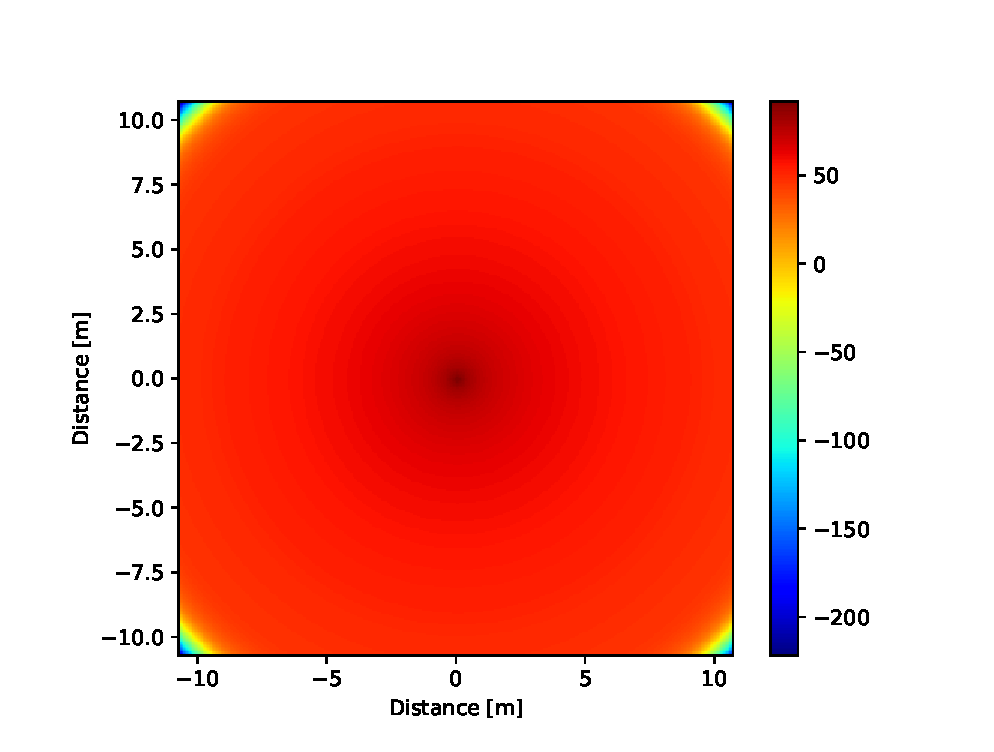
\includegraphics[width=1\textwidth]{p_rms_30m_64.eps}
\subcaption{$D=\SI{30}{\meter}$, double precision}
\label{fig:p_rms_30m_64}
\vspace{5mm}
\end{subfigure}
\caption{The figure shows the resulting \gls{rms} sound pressure level simulations with different grid sizes, where the caption for every figure specifies the grid size and the float precision}
		\label{fig:p_rms}
\end{figure}


